\section{Audit History and Estimand Map}
\label{sec:audit}

\paragraph{Corrections during preparation.} This paper was prepared under
an internal audit trail; three corrections are material to reading the
text. (i)~A transition-rate gap between screens was initially attributed
to crossing angle; a preregistered incidence analysis found no such law,
and the text retains only the screen-population explanation
(Sec.~\ref{sec:phenomenon}). That explanation does not say that unchanged
image information proves a sampling mechanism; the N02 comparison keeps
its MAC confound (App.~\ref{sec:f095}). (ii)~The P1G high-risk repair analysis
originally read dev thresholds through a stale key and silently fell back
to confirmation-pool quantiles; the analysis is re-run with the frozen dev
thresholds, and the residual-error statement in
Sec.~\ref{sec:phenomenon} carries the corrected numbers (re-run landed;
see R1 in \texttt{reports/caea817\_review/RECTIFICATION\_LOG.md}). (iii)~A
decision-interface calibration fit had a sign error; the corrected fit
replaces an earlier ``anti-information'' reading, and the interface
section reports coverage/precision decomposition only. Per-item
rectification records: \texttt{reports/caea817\_review/RECTIFICATION\_LOG.md}.

\paragraph{Estimand map.} The paper keeps two reliability notions
separated throughout: endpoint reliability (preserve/flip error over
unscreened starts) and conditional update reliability (both conditioned on
start correctness). $R(\tau, \rho)$ retention curves are
risk-reweightings of a retained population with mixing weight $\rho$,
not unselected deployment incidences; a bootstrap interval of $[1,1]$
reflects no observed variation in the retained set, not a population-level
proof of certainty. Where denominators differ across screens
($176$ vs $251$; $141$ vs $176$), contrasts are labeled descriptive.

\begin{figure}[t]
\centering
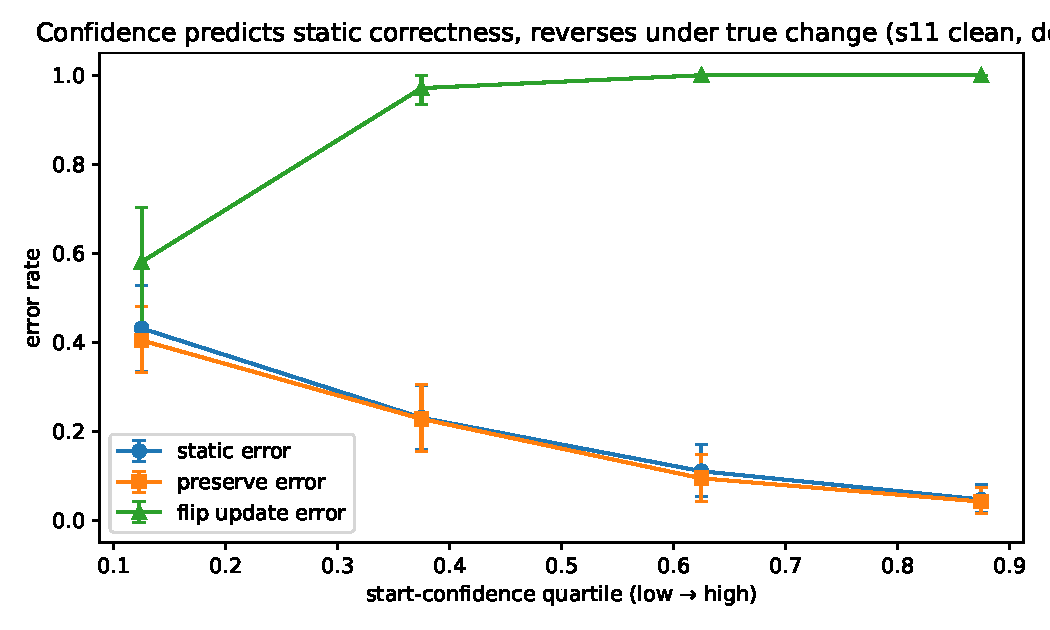
\includegraphics[width=0.9\linewidth]{figures/fig2_p1_dual.pdf}
\caption{Confidence versus static, preserve, and update error in one panel,
s11 clean on the dev bank; confirmation-bank curves show the same
separation. Three series with per-bin parent-cluster bootstrap intervals;
current-state error is computed over unscreened starts, update error
conditioned on start correctness. This coordinate-only side result is not
the repair-flow example in Fig.~\ref{fig:repair_examples}.}
\label{fig:p1}
\end{figure}

\paragraph{Domain change labels.} Coordinate scenes: synthetic controlled
edits. Football E2: controlled crossings constructed on real tracking
coordinates. Football natural turns: actual match events. Pixel:
controlled renders, one same-style replication plus four altered styles.
No cross-domain substitution is made between these categories.
